\section{Statement of Intent}

This was as far as I made it working on the problem in high school. I’ve set out this college semester (Junior year) to utilize the more advanced mathematics tools I have since learned to combat my old nemesis and finally ``slay the dragon'', so to speak. My research on this topic has consisted of three main goals:

\begin{enumerate}
    \item Given an arbitrary continuously differentiable function $y = f(x)$, I want to be able to predict exactly where all of its crunch spots are in $\mathbb{R}^2$.
    \item If possible I want to find a closed formula for the actual $N$-Units Away Curves.
    \item For each crunch spots, I’d like to come up with a formula for (or at least some scientific understanding of) the three paths that the vertices of each divot triangle follow as N increases.

\end{enumerate}

At this point in the reading of this paper, I would definitely recommend that my readers pause here for a little while and play around with $N$-Units Away Curves themselves! They’re really fun. Simply go to Desmos.com and type in the following equations. Note that to make a derivative you type in ``d/dt''. Also make sure to set the t bounds to something like $-10 \leq t \leq 10$.

\begin{figure}[ht]
  \centering
  \begin{minipage}[b]{0.8\linewidth}
  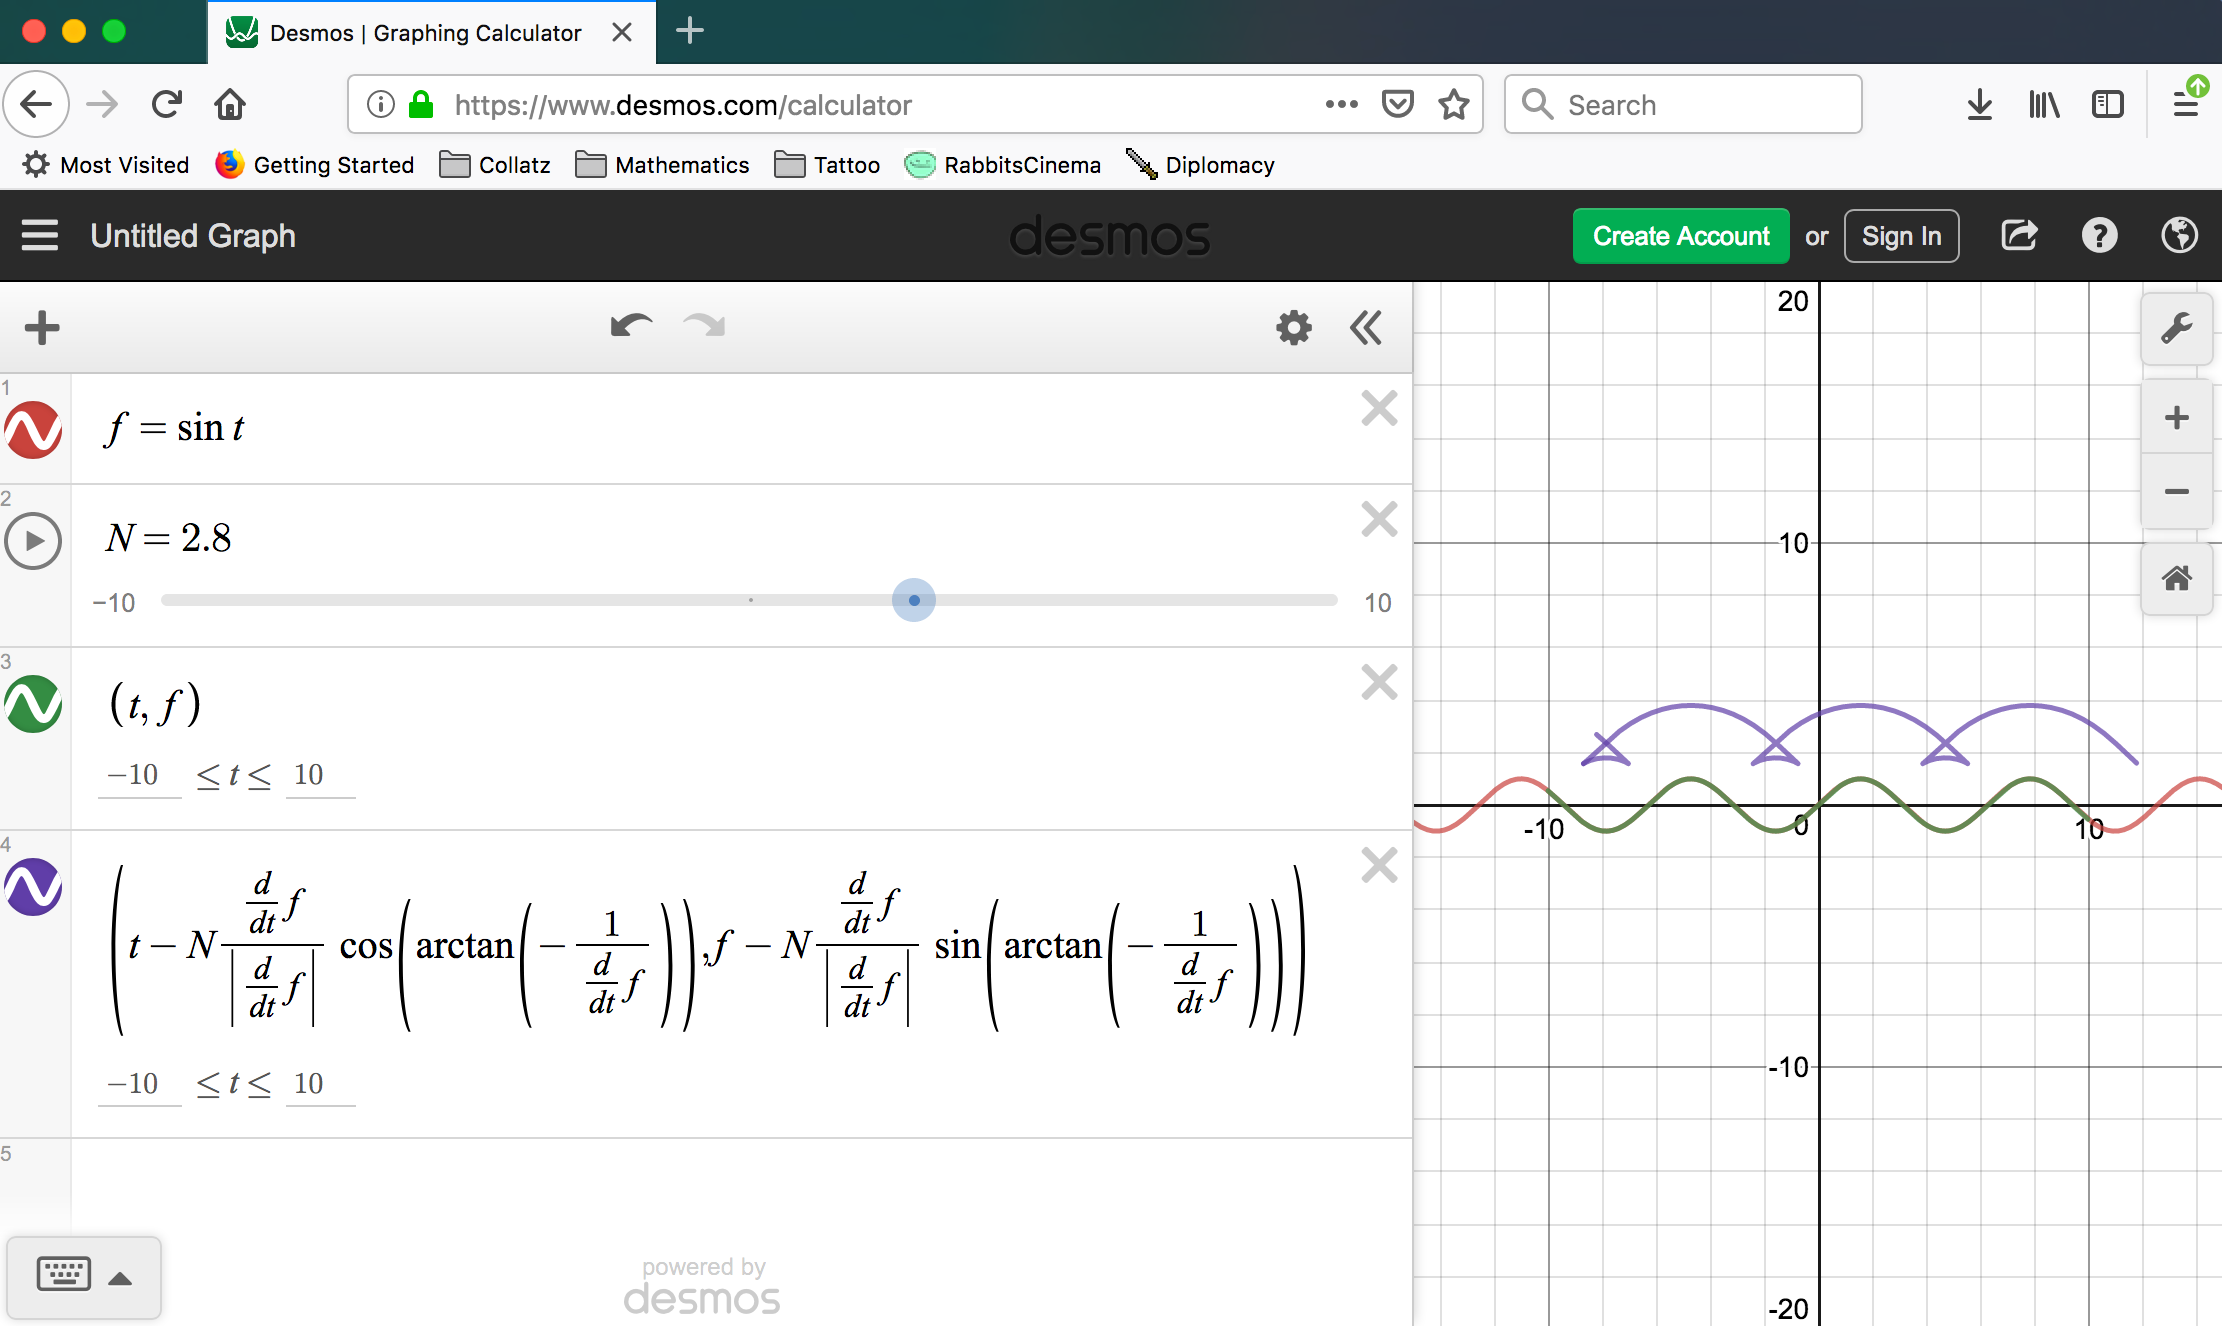
\includegraphics[width=\linewidth]{statement-of-intent-img/Desmos.png}
  \caption{Desmos | Graphing Calculator}
  \label{fig:desmos}
  \end{minipage}
\end{figure}

... Then change Equation 1 to whatever function you’d like and drag the slidable $N$ value to
observe the behavior of the $N$-Units Away Curves. Have fun!

Now let’s get down to business...